\section{Modelling the shear correlation functions}
\label{sec:xipm}
A convenient way to infer cosmological information from observational data are the shear correlation functions $\xi_\pm$, which are defined as \[
\xi_\pm = \la \gamma_{\rm t}\gamma_{\rm t}\ra \pm \la \gamma_\times\gamma_\times\ra \, .
\]
They are the prime estimators to quantify a cosmic-shear signal since it is simple to include a weighting of the shear-measurements into the correlation functions and, contrary to the power spectrum, one does not have to worry about the shape of the survey footprint, or masked regions. Cosmologically, given two comoving distance probability distributions of sources $p_i(\chi),p_j(\chi)$, one can compute the shear correlation function from the underlyting matter power spectrum $P_\delta$ via \todo{Citation!}\begin{align}
\label{eq:xipm-pkappa}
\xi_\pm[\theta,p_i,p_j] =& \int_0^\infty \frac{{\rm d}l\,l}{2\pi}J_{0,4}(l\theta)P(l,p_i,p_j)\, , \\
\label{eq:pkappa-pdelta/lenseff}
P(l,p_i,p_j) =& \frac{9 H_0^4\Omega_{\rm m}^2}{4c^4}\int_0^{\chi_h} {\rm d}\chi\frac{g(\chi,p_i)g(\chi,p_j)}{a^2(\chi)}P_\delta\left(\frac{l}{f_K(\chi)},\chi\right)\, , \\
\label{eq:lenseff}
g(\chi,p_i) =& \int_\chi^{\chi_H} {\rm d}\chi'\, p_i(\chi') \frac{f_K(\chi'-\chi)}{f_K(\chi')}\, .
\end{align}
Here, $J_{0,4}$ denote the 0-th and 4-th order Bessel Functions.
\subsection{Using an analytic Model}
For a first simple analysis we will assume that a deeper redshift distribution just yields a stronger shear signal. Following \citet{2006APh....26...91V}, we estimate
\[
\la |\gamma| \ra \propto \la z \ra ^{0.85}\, .
\]
\todo{Maybe implement redshift-dependent index?}
Additionally, we assume that a higher depth does not only lead to a stronger average shear, but also to a higher galaxy number density, implying a correlation between those two quantities.

%For a pair of galaxies that we use to measure the correlation function, it is crucial to determine whether those two galaxies lie within the same pointing. We want to define a function $E(\theta)$ that determines 

Let $N(\b \theta)$ be the number-density per tile and $W(\b \theta)$ the weighting of average shear. The observed correlation function $\xi^{\text{obs}}_\pm(\theta)$ now changes from one of constant depth $\xi_\pm^{\rm const}$ via 
\begin{align*}
\xi^{\text{obs}}_\pm(\theta) = & \frac{\la N(\b 0)N(\b \theta)\gammao_{\rm t}(\b 0)\gammao_{\rm t}(\b \theta)\ra }{\la N(\b 0)N(\b \theta)\ra} \pm \frac{\la N(\b 0)N(\b \theta)\gammao_\times(\b 0)\gammao_\times(\b \theta)\ra }{\la N(\b 0)N(\b \theta)\ra} \\
 = & \frac{\la N(\b 0)N(\b \theta)W(\b 0)W(\b \theta)\ra}{\la N(\b 0)N(\b \theta)\ra} \xi_{\pm}^{\rm const}(\theta) \, .
 \end{align*}
 Assuming that depth and galaxy number density of neighbouring pointings are uncorrelated, the only important property of a galaxy pair is whether or not they lie in the same pointing. We want to denote the probability that a random pair of galaxies of distance $\theta$ lie in the same pointing with $E(\theta)$. This function can be calculated as in Appendix \ref{sec:details on etheta} and equates to
\begin{equation}
E(\theta) =  \begin{cases}
\frac{1}{L^2 \pi}\left[L^2\pi - (4L-\theta) \theta\right]\, ,  & \theta \leq L \\[10pt]
\frac{2}{\pi}\,\left[4\sqrt{\frac{\theta^2}{L^2}-1} -1 - \frac{\theta^2}{2L^2} - \cos\inv\left(\frac{L}{\theta}\right) + \sin\inv\left(\frac{L}{\theta}\right)\right]\, ,  & L  \leq \theta \leq \sqrt{2}L \\[10pt]
0\, ,  & \sqrt{2}L \leq \theta
\end{cases}\, .
\end{equation} 
 This function is depicted in Figure \ref{fig:eoftheta_lin}. 
 
 \begin{figure}
 \centering
 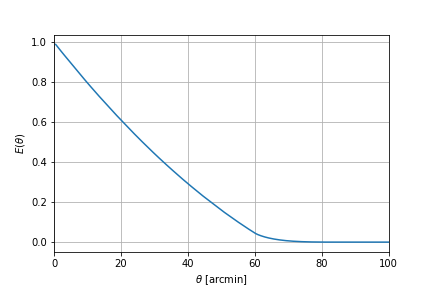
\includegraphics[width=0.5\textwidth]{images/eoftheta.png}
 \caption{Probability that a random pair of galaxies of distance $\theta$ lie in the same pointing.}
 \label{fig:eoftheta_lin}
 \end{figure}

We again parametrize the number density $N(\b \theta)=\la N \ra (1+n(\b \theta))$ and the weight $W(\b \theta)=1+w(\b \theta)$ and, as in \eqref{eq:defweightf}, interpret $n(\b \theta)$ as a locally constant function with average $\la n \ra = 0$. We can see that $\la n(\b 0)n(\b \theta)\ra = E(\theta)\la n(\b 0)n(\b 0)\ra \equiv E(\theta)\la n n \ra$ holds and get for the autocorrelation of a single bin, 
 \begin{align}
\xi^{\text{obs}}_\pm(\theta) = & \frac{1 + 2\la nw \ra + E(\theta)\left[\la (n+w)^2\ra + 2 \la n^2 w\ra + 2\la nw^2\ra + \la n^2 w^2\ra \right]}{1+E(\theta)\la n^2\ra }\xi_\pm^{\rm const}(\theta) \\
\approx & \frac{1 + 2\la nw \ra + E(\theta)\left[\la (n+w)^2\ra \right]}{1+E(\theta)\la n^2\ra }\xi_\pm^{\rm const}(\theta)\, , \nonumber
 \label{eq:ffunct}
\end{align}
holds. We see that in addition to a modification of the correlation function due to the stronger shear signal in deeper pointings, we also get a scale-independent modification due to the correlation between depth and number density.

However, as a survey of constant depth is completely unrealistic, also the modelled correlation function will be subject to the same effect. If we assume the same redshift-distributions for galaxies as in the case of varying depth, and just assert that those changes are not correlated with position, we get 
\begin{equation}
\xi_\pm = (1+2\la nw\ra)\xi_\pm^{\rm const}\, .
\end{equation}
The ratio of modelled and observed correlation function thus becomes: \begin{align}
\frac{\xi_\pm}{\xi_\pm^{\rm obs}} = & \frac{\left(1+2\la nw\ra\left)\left(1+E(\theta)\la n^2\ra\right)\right.\right.}{1 + 2\la nw \ra + E(\theta)\left[\la (n+w)^2\ra + 2 \la n^2 w\ra + 2\la nw^2\ra + \la n^2 w^2\ra \right]} \\
\equiv & F(\theta) \, .
\end{align}
A similar, but longer, equation governs the cross-correlation between different bins. This equation and its derivation can be found in Appendix \todo{create this and cite it.}.
%It is interesting to note that $F(\theta)=1$ holds wherever $E(\theta)=0$, meaning that the correlation function is not affected for large angular scales. 
We shall later see that this approximation is valid for higher tomographic redshift bins $z\gtrsim 0.5$, but starts to break down at lower redshifts. 
\subsection{Using a semi-analytic Model}
The analysis of data from the Kilo-Degree Survey showed that the redshift-distribution of sources was highly correlated with the depth in the $r$-band. We thus chose to separate the survey into 10 percentiles, sorted by $r$-band depth, meaning that if a pointing had a worse depth than 90\% of the other pointings, it would belong to the first percentile, and so on. Now for each percentile $m$ and each tomographic redshift bin $i$ we can extract a weighted number of galaxies $N^i_m$ and, in case the pointing overlaps with a spectroscopic survey, a source redshift distribution $p^i_m(z)$. Using \eqref{eq:xipm_from_pkappa}, we can compute the shear correlation functions $\xi_{\pm,mn}^{ij}(\theta)$ for each set of percentiles $m,n$ and redshift bins $i,j$\footnote{For the calculation of the shear correlation functions we use the \textsc{Nicaea}-program. Among other things, it calculates the shear correlation functions for a given cosmology and source redshift distribution. To estimate the power spectrum on nonlinear scales we use the methods developed by \citet{2012ApJ...761..152T}.}. When we compute the measured shear correlation functions of a survey, we take the weighted average of tangential and cross shears of all pairs of galaxies (\citet{2017MNRAS.465.1454H} give a good overview for the process). If, for a single pair of galaxies, one galaxy lies in the $m$-th percentile of redshift bin $i$ and the second one lies in the $n$-th percentile of redshift bin $j$, then their contribution to the observed correlation functions is, on average, $\xi_{\pm,mn}^{ij}(\theta)$. This means that if we know each of those single correlation functions, we can reconstruct the total correlation functions via a weighted average of the single functions. Formally, we define \[
\xi_\pm^{ij,\rm{obs}}(\theta) = \frac{\sum_{m,n} P_{mn}^{ij}(\theta)\xi_{\pm,mn}^{ij}(\theta)}{\sum_{m,n} P_{mn}^{ij}(\theta)}\, ,
\label{eq:def_xiobs}
\]
where $P_{mn}^{ij}$ is the new weighting of the correlation functions. This weighting has to be proportional to the probability that a galaxy pair of distance $\theta$ is of percentiles $m$ and $n$, as well as to the original weighting of these galaxies.\todo{We could completely scratch this derivation and just point to the Appendix; I personally feel that this approach is more intuitive than the more mathematical one of the appendix, but if the paper gets too long we definitely do not need two methods to derive the same equation.}

In this analysis, we will assume an infinitely large survey footprint with an uncorrelated distribution of depth. We will later discuss the validity of these assumptions as well as possible mitigation strategies. For $m\neq n$ we know that the pair of galaxies has to lie in different pointings, which is accounted for by including the factor $[1-E(\theta)]$. Furthermore, the first galaxy has to lie in percentile $m$, the probability of which is $1/10$. When the first pointing is of percentile $m$, the probability that a galaxy in a different pointing is of percentile $n$ is also equal to $1/10$. The impact of such a galaxy pair on the correlation functions scales with the product of the weighted number of galaxies $N_m^i,N_n^j$. We get for $n\neq m$: \[
P_{mn}^{ij}(\theta) = [1-E(\theta)]\frac{1}{100} N_m^i N_n^j\, .
\label{eq:pmnij_corr1}
\]
For the calculation of $P_{mm}^{ij}(\theta)$ we have to account for a different possibility: In case that the galaxy lies in the same pointing [accounted for by the factor $E(\theta)$], it automatically is of the same percentile. We therefore set \[
P_{mm}^{ij}(\theta) = E(\theta)\frac{1}{10} N_m^iN_m^j + [1-E(\theta)]\frac{1}{100} N_m^i N_m^j \, .
\label{eq:pmnij_corr2}
\]
We can then write $P_{mn}^{ij}(\theta)$ as: \[
P_{mn}^{ij}(\theta) = E(\theta)\frac{1}{10} N_m^iN_n^j\,\delta_{mn} + [1-E(\theta)]\frac{1}{100} N_m^i N_m^j \, ,
\label{eq:pmnij_uncorr}
\]
where $\delta_{mn}$ denotes the Kronecker delta.
Inserting this into Eq.\,\eqref{eq:def_xiobs}, we compute
\begin{align}
\xi_{\pm,mn}^{ij,\rm{obs}}(\theta) = & \frac{1}{C}\sum_{m=1}^{10} N_m^i \left\{ E(\theta) N_m^j \xi_{\pm,mm}^{ij}(\theta) + \frac{\big[1-E(\theta)\big]}{10}\sum_{n=1}^{10}N_n^j \xi_{\pm,mn}^{ij}(\theta)\right\}\, ,
\label{eq:correctionfunction1}
\end{align}
with the normalization
\[
C = \sum_{m=1}^{10} N_m^i \bigg[ E(\theta)  N_m^j + \frac{\big[1-E(\theta)\big]}{10}\sum_{n=1}^{10} N_n^j\bigg]\, .
\]
A more mathematically rigorous derivation of this function can be found in Appendix \ref{sec:calc of xipm}.

If we want to compute this for all 5 redshift bins of the KV450-survey, this forces us to calculate 1275 correlation functions and add them, thus yielding potential numerical errors (apart from being computationally expensive). However, if we examine Eq.\,\eqref{eq:lenseff}, we see that the comoving distance distribution of sources factors in linearly. This in turn implies that in Equations \eqref{eq:pkappa-pdelta/lenseff} and \eqref{eq:xipm-pkappa} both source distance distributions factor in linearly. This basically means that, instead of adding correlation functions, we can add their respective redshift distributions and compute the correlation functions of that. In particular, we can define the \textit{combined number of galaxies} $N^i$ and \textit{average redshift distribution} $p^i(z)$ of tomographic bin $i$ as \[
N^i\equiv\sum_m N_m^i\, , \qquad p^i(z) = \frac{\sum_m N_m^i p_m^i(z)}{\sum_m N_m^i} \, .
\]
If we define $\xi^{ij}_\pm$ as the correlation functions between the average redshift distributions $p^i(z)$ and $p^j(z)$, then we observe: \[
\sum_{m,n}N_m^iN_n^j\xi^{ij}_{\pm,mn} = N^iN^j\xi^{ij}_\pm\, .
\]
Consequently, we can apply this to \eqref{eq:correctionfunction1}, yielding
\begin{equation}
\xi_{\pm}^{ij,\rm{obs}}(\theta) = \frac{1}{C}\left\{ E(\theta)\left[\sum_{m=1}^{10} N_m^iN_m^j \xi_{\pm,mm}^{ij}(\theta)\right] +\frac{\big[1-E(\theta)\big]}{10}\xi_\pm^{ij}(\theta)N^iN^j\right\}\, .
\label{eq:correctionfunction2}
\end{equation}
For each set of redshift bins we thus only have to compute eleven correlation functions, which reduces the number of functions to compute from 1275 to 165. We can see that for large distances $\theta$, such that $E(\theta)=0$ holds, we have $C=N^iN^j$ and thus \[
\xi_{\pm}^{ij,\rm{obs}}(\theta) = \frac{1}{N^iN^j}\xi_\pm^{ij}(\theta)N^iN^j = \xi_\pm^{ij}(\theta)\, ,
\]
so on large scales our observed correlation functions agree with the ones that we would usually calculate.
